\documentclass[12pt,a4paper]{article}

% ---- Packages ----
\usepackage[utf8]{inputenc}
\usepackage[T1]{fontenc}
\usepackage{geometry}
\geometry{margin=1in}
\usepackage{setspace}
\usepackage{enumitem}
\usepackage[table]{xcolor}
\usepackage{array}
\usepackage{graphicx}
\graphicspath{{image/}}
\usepackage{hyperref}
\hypersetup{
    colorlinks=true,
    linkcolor=blue,
    urlcolor=blue,
    citecolor=blue
}
\usepackage{booktabs}
\usepackage{caption}
\usepackage{subcaption}
\usepackage{amsmath}
\usepackage{listings}
\usepackage{tikz}
\usetikzlibrary{arrows.meta, positioning}
\usepackage{fancyhdr}
\usepackage{etoolbox} % For \preto
\usepackage{titlesec} % For custom chapter titles

% Automatically start each section on a new page
\preto{\section}{\clearpage}

% Header and Footer setup (Removed the top rule line)
\setlength{\headheight}{15pt}
\pagestyle{fancy}
\fancyhead{}
\fancyfoot[C]{\thepage}
\renewcommand{\headrulewidth}{0pt}

% Section formatting to display "Chapter X: Title"
\titleformat{\section}
  {\normalfont\Large\bfseries}
  {Chapter \thesection:}
  {0.5em}
  {}

\definecolor{kublue}{RGB}{0, 85, 164}
\definecolor{lightblue}{RGB}{235, 243, 250}
\definecolor{codebg}{rgb}{0.95,0.95,0.95}

\lstset{
    basicstyle=\footnotesize\ttfamily,
    backgroundcolor=\color{codebg},
    frame=single,
    breaklines=true,
    numbers=left,
    numberstyle=\tiny,
}

\begin{document}

% ---- 1. Cover Page ----
\begin{titlepage}
\setstretch{1.5}
\centering

\vspace*{0.5cm}
\textbf{\Large Kathmandu University}\\
\textbf{\large Department of Computer Science and Engineering}\\
\textbf{\large Dhulikhel, Kavrepalanchowk}

\vspace{1.2cm}


\includegraphics[width=4.5cm]{image/ku_logo.png}

\vspace{1.2cm}

\textbf{\large A Mini Project on}\\
\vspace{0.3cm}
\textbf{\Large ``Hands-Free PC Control Using Acoustic Gestures \\(STEC v2)''}\\
\vspace{0.4cm}
\textbf{\large [Code No: COMP 407]}

\vspace{1.5cm}

\textbf{Submitted by:}\\
Prabin Aryal (08)\\
Dikshit Bhatta (13)

\vspace{1cm}

\textbf{Submitted to:}\\
Mr. Rupesh Dahi Shrestha\\
Department of Computer Science and Engineering

\vspace{\fill}

\textbf{Submission Date:} 2026/07/04

\vspace*{0.5cm}
\end{titlepage}

\newpage

% ---- 2. Abstract ----
\section*{Abstract}
\addcontentsline{toc}{section}{Abstract}
This report describes the design, implementation and evaluation of a real-time acoustic gesture recognition system that uses transient sounds (finger snaps, hand claps and tongue clicks) as hands-free input triggers for OS-level macros. The system uses a second-generation Spectro-Temporal Envelope Correlation (STEC) pipeline: a 12-band log-spaced SOS Butterworth filterbank extracts sub-band energy envelopes from onset-aligned audio windows; these are noise-floor-subtracted, log-compressed, augmented with temporal delta features and L2-normalised to produce a volume-invariant 2D structural fingerprint. Multi-exemplar template matching with discriminative cosine-similarity rejection drives classification. A guarded EMA-based adaptation mechanism adjusts templates on high-confidence hits. A gesture-sequence state machine handles chained trigger patterns and a macro engine dispatches hotkeys, text, URLs, shell commands and application launches. An offline synthetic test suite evaluates the pipeline across noise conditions from 0 to 30 dB SNR, a 40 dB gain sweep, distractor rejection and confusion analysis. The system achieves 86.7\% classification accuracy at 15 dB SNR with a 3.3\% false-positive rate and zero inter-gesture confusions in the confusion matrix. The system is implemented in Python with a PyQt6 graphical interface and real-time audio capture via PortAudio.

\newpage

% ---- Table of Contents ----
\tableofcontents
\newpage

% ---- 3. Introduction ----
\section{Introduction}

\subsection{Theoretical Background}

Acoustic transient detection uses digital signal processing techniques to identify brief, broadband sound events in continuous audio streams. The core problem is distinguishing intentional transient sounds (finger snaps, hand claps and tongue clicks) from background noise and other acoustic activity. These transients have rapid onset, wide spectral content and rapid decay. This makes them distinct from sustained sounds or gradual noise.

Machine-based detection requires a multi-stage pipeline. Early work in acoustic transient processing, such as the neuromorphic architecture proposed by Pineda et al.~\cite{pineda1996}, established a template of time-frequency analysis followed by rectification, smoothing and template correlation. Later work by Bello et al.~\cite{bello2005} provided a taxonomy of onset detection methods and showed that spectral flux (the frame-to-frame difference in magnitude spectra) is effective for percussive transient detection.

The STEC algorithm combines a log-spaced filterbank with sub-band envelope extraction and cosine-similarity template matching. The pipeline works as follows: a filterbank separates the audio into frequency bands; each band is rectified and smoothed to extract the energy envelope; the resulting multi-band profile is normalised and compared against stored templates. Schroder et al.~\cite{schroder2015} found that filterbank-based spectro-temporal features outperform MFCCs for acoustic event detection.

\subsection{Background and Motivation}

Hands-free human-computer interaction addresses scenarios where hands are occupied during cooking, driving, medical procedures or accessibility use cases. Voice control carries privacy concerns in shared spaces and performs poorly in high-noise environments. Acoustic gesture recognition using transient sounds presents an alternative. Snaps, claps and clicks are broadband and can be produced without speech.

Current commercial solutions rely on voice assistants (Amazon Alexa, Google Assistant, Apple Siri) or camera-based gesture recognition (Microsoft Kinect, Leap Motion). Voice control streams audio to cloud services and degrades in loud environments. Camera-based systems need dedicated hardware and line-of-sight. Acoustic transient recognition requires only a standard microphone and operates offline. Because transients are broadband they can be distinguished from narrowband background noise.

The central technical challenge is developing a system that operates reliably across varied acoustic conditions. The same gesture from the same person varies in amplitude, spectral detail and timing across repetitions. Background noise changes. The system must reject unknown sounds rather than triggering on them. This work addresses these problems using a STEC v2 pipeline with scale-relative adaptive thresholding, noise-floor compensation, discriminative margin-based rejection and guarded adaptive learning.

\subsection{Purpose}

The purpose of this project is to design and implement a real-time acoustic gesture recognition system that:

\begin{enumerate}
    \item Detects percussive transient sounds (snaps, claps, clicks) from a standard microphone across varying noise conditions.
    \item Classifies the detected gesture and rejects unknown sounds with a low false-positive rate.
    \item Maps recognised gestures to OS-level macros (hotkeys, text input, URL opening, application launching, shell commands).
    \item Provides a graphical interface for training new gestures, configuring macro mappings and visualising the DSP pipeline in real time.
    \item Adapts to the user's environment over time without manual recalibration.
\end{enumerate}

% ---- 4. Problem Statement ----
\section{Problem Statement}

Current hands-free computer interaction paradigms are largely limited to voice control and camera-based gesture recognition. Voice assistants need internet connectivity and perform poorly in noise. Camera-based systems require dedicated hardware and a line-of-sight path.

Acoustic transient-based gesture recognition (using sounds such as finger snaps and hand claps) can address these limitations. However, existing implementations exhibit several shortcomings:

\begin{enumerate}
    \item \textbf{Volume sensitivity:} Energy-threshold-based onset detectors fail when the same gesture is performed at different volumes. A quiet snap remains undetected; a loud clap triggers erroneously on the reverberation tail.
    \item \textbf{Noise vulnerability:} Background noise varies across environments. Fixed thresholds cannot adapt.
    \item \textbf{False positives:} Unknown sounds (door slams, keyboard clicks, speech) may be mistaken for trained gestures.
    \item \textbf{Template rigidity:} Single-template matching does not account for natural variation between repetitions of the same gesture.
    \item \textbf{Environmental drift:} A system calibrated in one environment degrades as room acoustics or background noise change.
    \item \textbf{Limited integration:} Existing academic solutions rarely connect to OS-level actions.
\end{enumerate}

This project addresses each of these problems through a redesign of the STEC pipeline, described in the following sections.

% ---- 5. Methodology ----
\section{Methodology}

\subsection{System Architecture Overview}

The system uses a streaming pipeline. Audio is captured from the microphone via a \texttt{sounddevice.InputStream} with a ring buffer. A spectral-flux onset detector continuously analyses the stream. When it locates a transient, an onset-aligned window is cut from the ring buffer and sent to the STEC feature extractor. The resulting structural fingerprint is compared against a multi-exemplar template library via cosine similarity. If the best-matching gesture clears a similarity threshold and a discriminative margin against the runner-up, it is appended to a gesture-sequence state machine. When the accumulated sequence matches a user-configured mapping, the corresponding macro fires.

The signal-processing chain is:

\begin{figure}[ht]
\centering
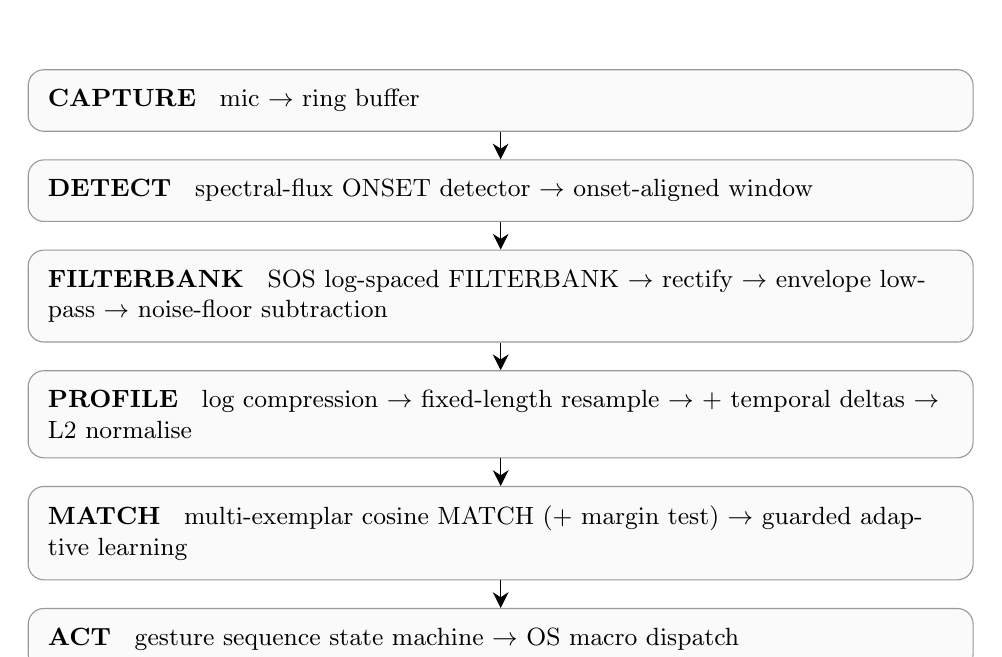
\begin{tikzpicture}[
    phase/.style={draw=black!40, rounded corners=2mm, text width=11.5cm, align=left, inner sep=2.5mm, font=\small},
    >={Stealth[width=2mm, length=2mm]},
]
\node[phase, fill=gray!4] (p1) {%
\textbf{CAPTURE}\hspace{0.3cm}%
mic $\rightarrow$ ring buffer%
};
\node[phase, fill=gray!4, below=0.35cm of p1] (p2) {%
\textbf{DETECT}\hspace{0.3cm}%
spectral-flux ONSET detector $\rightarrow$ onset-aligned window%
};
\node[phase, fill=gray!4, below=0.35cm of p2] (p3) {%
\textbf{FILTERBANK}\hspace{0.3cm}%
SOS log-spaced FILTERBANK $\rightarrow$ rectify $\rightarrow$ envelope lowpass $\rightarrow$ noise-floor subtraction%
};
\node[phase, fill=gray!4, below=0.35cm of p3] (p4) {%
\textbf{PROFILE}\hspace{0.3cm}%
log compression $\rightarrow$ fixed-length resample $\rightarrow$ + temporal deltas $\rightarrow$ L2 normalise%
};
\node[phase, fill=gray!4, below=0.35cm of p4] (p5) {%
\textbf{MATCH}\hspace{0.3cm}%
multi-exemplar cosine MATCH (+ margin test) $\rightarrow$ guarded adaptive learning%
};
\node[phase, fill=gray!4, below=0.35cm of p5] (p6) {%
\textbf{ACT}\hspace{0.3cm}%
gesture sequence state machine $\rightarrow$ OS macro dispatch%
};
\draw[->, thin] (p1) -- (p2);
\draw[->, thin] (p2) -- (p3);
\draw[->, thin] (p3) -- (p4);
\draw[->, thin] (p4) -- (p5);
\draw[->, thin] (p5) -- (p6);
\end{tikzpicture}
\caption{STEC v2 signal-processing pipeline.}
\label{fig:pipeline}
\end{figure}

\subsection{Continuous Ring Buffer}

Audio accumulates in a rolling ring buffer of length \(0.75 \times f_s\) samples. The analysis window is taken from this buffer rather than from individual audio callbacks, ensuring that a transient landing between callbacks is neither missed nor truncated. The buffer is a fixed-size NumPy array with a rolling write pointer.

\subsection{Spectral-Flux Onset Detection}

Transient detection uses an HFC-weighted spectral-flux onset detection function (ODF). This is more selective for percussive transients than a raw energy threshold and tolerates slow changes in background noise.

The ODF is:

\[
\text{ODF}[n] = \sum_{k} \max\left(0,\, |X_n[k]| - |X_{n-1}[k]|\right) \cdot w[k]
\]

where \(X_n[k]\) is the \(n\)-th STFT frame and \(w[k] = 0.3 + 0.7 \cdot (k / K_{\text{max}})\) applies soft high-frequency emphasis.

A scale-relative adaptive threshold is used for peak-picking:

\[
\theta[i] = \max\left(\theta_{\min},\; \mu_{\text{local}}[i] + k \cdot \sigma_{\text{local}}[i]\right)
\]

where \(\mu_{\text{local}}\) and \(\sigma_{\text{local}}\) are the mean and standard deviation of the ODF over a local neighbourhood of 11 frames, and \(k = 2.5\). The threshold collapses to \(\theta_{\min}\) in near-silence (where \(\sigma \rightarrow 0\)). Transient peaks clear the adaptive floor regardless of absolute loudness, therefore detection is volume-invariant.

\subsection{SOS Log-Spaced Filterbank}

The audio is routed through 12 log-spaced Butterworth band-pass filters from 500 Hz to 12 kHz. Each filter is 4th-order, implemented as second-order sections (SOS). High-order Butterworth band-passes at 44.1 kHz are numerically unstable in transfer-function \((b, a)\) form because poles cluster near the unit circle. SOS decomposition with forward-backward filtering (\texttt{sosfiltfilt}) gives clean, phase-free sub-band envelopes.

The band edges follow a logarithmic spacing:

\[
f_i = \log_{10}^{-1}\left( \log_{10}(f_{\text{low}}) + i \cdot \frac{\log_{10}(f_{\text{high}} / f_{\text{low}})}{N} \right), \quad i = 0 \dots N
\]

\subsection{Structural Profiling}

For each detected transient, an onset-aligned window is extracted (30 ms pre-onset, 120 ms post-onset) and processed through:

\begin{enumerate}
    \item \textbf{Sub-band envelope extraction:} Each band-pass filter is applied via zero-phase SOS filtering, then full-wave rectified and low-pass filtered at 50 Hz (also SOS).

    \item \textbf{Noise-floor subtraction:} The 15th percentile of each band's envelope is subtracted before further processing. This removes the flat pedestal so the log stage does not amplify background noise in bands without transient energy. Without this step, low-frequency clap energy leaks into high-band click templates.

    \item \textbf{Log compression:} Each band is resampled to 64 fixed time frames and log-compressed:
    \[
    \hat{e}_b[t] = \log\left(1 + \gamma \cdot e_b[t]\right), \quad \gamma = 30
    \]
    where \(\gamma\) controls the compression gain.

    \item \textbf{Temporal deltas:} First-order temporal differences are appended as additional feature rows:
    \[
    \Delta_b[t] = \hat{e}_b[t] - \hat{e}_b[t-1]
    \]
    These capture attack/decay dynamics. The feature dimensionality becomes \(2N_{\text{bands}} \times 64\).

    \item \textbf{L2 normalisation:} The feature vector is L2-normalised:
    \[
    \mathbf{f} \leftarrow \frac{\mathbf{f}}{\|\mathbf{f}\|_2}
    \]
    This bounds cosine similarity and makes it volume-invariant.
\end{enumerate}

\subsection{Multi-Exemplar Template Matching}

During training, a 3-second recording of a gesture is segmented into every transient it contains using the same onset detection function as at run time. Each transient window is profiled independently, giving multiple \textit{exemplars} per gesture. A mean profile is computed via L2-normalised element-wise averaging.

At run time, a live profile is scored against all gestures using nearest-exemplar cosine similarity:

\[
\text{score}(g) = \max_{e \in \mathcal{E}_g} \, \langle \mathbf{f}_{\text{live}}, \mathbf{f}_e \rangle
\]

where \(\mathcal{E}_g\) includes both exemplars and the mean template for gesture \(g\).

\subsection{Discriminative Rejection}

A gesture is accepted only when both conditions hold:

\[
\text{score}_{\text{best}} \geq \tau_s \quad \text{and} \quad (\text{score}_{\text{best}} - \text{score}_{\text{second}}) \geq \tau_m
\]

where \(\tau_s = 0.75\) is the similarity threshold and \(\tau_m = 0.05\) is the rejection margin. The margin test reduces false positives because unknown sounds may have moderate similarity to a gesture but rarely produce sufficient separation.

\subsection{Guarded Adaptive Learning}

Templates update via exponential moving average (EMA) blending, but only on hits that meet stricter criteria:

\[
\tau_{\text{adapt}} = 0.85, \quad \tau_{m,\text{adapt}} = 0.10
\]

When these are satisfied, the matched exemplar is blended:

\[
\mathbf{f}_{e} \leftarrow (1 - \alpha) \cdot \mathbf{f}_{e} + \alpha \cdot \mathbf{f}_{\text{live}}, \quad \alpha = 0.15
\]

followed by re-normalisation. Adapting the nearest exemplar (instead of a single global template) preserves the intra-gesture diversity from training.

\subsection{Gesture Sequence State Machine}

A two-state machine (IDLE / ARMED / EXECUTE) handles chained sequences. After a recognised gesture, the system enters ARMED and waits for a second gesture within a configurable timeout (3 seconds). If the accumulated sequence matches a user-defined mapping, the state transitions to EXECUTE and the corresponding macro fires. The sequence is pruned when it can no longer form a prefix of any registered mapping.

% ---- 6. Implementation ----
\section{Implementation (Code/Simulation)}

The system is implemented in Python 3.14, with a modular architecture separating DSP core, GUI and configuration.

\subsection{Project Structure}

The codebase is organised as:

\begin{lstlisting}
DSP miniproj/
  main.py                  # Application entry point
  config.py                # All tunable parameters
  test_stec.py             # Offline synthetic test suite
  core/
    audio_streamer.py      # PortAudio microphone capture
    calibration_engine.py  # STEC feature extraction + training
    event_detector.py      # Streaming detection + state machine
    dsp_utils.py           # Filter design, spectral flux, peak-picking
    macro_executor.py      # Macro dispatch engine
    macro_store.py         # Custom macro persistence
  gui/
    main_window.py         # PyQt6 main window layout
    calibration_panel.py   # Gesture recording and mapping UI
    visualizer_panel.py    # Real-time waveform/spectrum/ODF/heatmap
    console_panel.py       # Timestamped event log
    macro_dialog.py        # Custom macro creation dialog
  assets/
    style.qss              # GitHub Dark-inspired stylesheet
  Report/
    report.tex             # This document
    image/                 # Figures and KU logo
\end{lstlisting}

\subsection{DSP Core Modules}

The DSP pipeline is implemented across four core modules.

\texttt{dsp\_utils.py} provides stateless primitives: Butterworth filterbank design as second-order sections, envelope lowpass filter design, spectral-flux ODF computation using vectorised STFT framing and scale-relative adaptive peak-picking using local mean and standard deviation.

\texttt{calibration\_engine.py} implements the \texttt{SpectroTemporalProfiler} class, which manages the filterbank, feature extraction from onset-aligned windows, multi-exemplar template storage, cosine-similarity matching and guarded EMA-based template adaptation. The pipeline from window to profile is:

\begin{lstlisting}[language=Python]
def profile_from_window(self, window):
    # 1. SOS bandpass filterbank
    # 2. Rectify + SOS lowpass envelope
    # 3. 15th percentile noise-floor subtraction
    # 4. Resample to 64 frames + log1p compression
    # 5. Optional temporal delta rows
    # 6. L2 normalise
    return profile
\end{lstlisting}

\texttt{event\_detector.py} implements the \texttt{EventDetector} class, which maintains the ring buffer, runs the spectral-flux ODF on every chunk, performs onset peak-picking, classifies transients through the profiler and manages the gesture-sequence state machine. The cooldown mechanism is sample-based (not wall-clock-based), so behaviour is identical in live and offline settings.

\texttt{audio\_streamer.py} wraps \texttt{sounddevice.InputStream} with a thread-safe queue for non-blocking capture. It uses lazy imports so the DSP core works without audio hardware.

\subsection{Macro Engine}

The macro executor supports eight action types (Table~\ref{tab:macro-types}). Each macro is a dictionary with a type field and type-specific payload.

\begin{table}[h]
\centering
\caption{Supported macro action types.}
\label{tab:macro-types}
\begin{tabular}{@{}lll@{}}
\toprule
Type & Payload & Example \\
\midrule
\texttt{hotkey} & \texttt{keys} list & \texttt{ctrl+alt+t} \\
\texttt{press}  & \texttt{keys} list & \texttt{playpause} \\
\texttt{text}   & \texttt{value} string & \texttt{my.email@x.com} \\
\texttt{url}    & \texttt{value} string & \texttt{https://chatgpt.com} \\
\texttt{open}   & \texttt{value} path  & \texttt{$\sim$/Downloads} \\
\texttt{launch} & \texttt{value} command & \texttt{code .} \\
\texttt{shell}  & \texttt{value} command & \texttt{notify-send `Snap!'} \\
\texttt{sequence} & \texttt{actions} list & chained sub-actions with delays \\
\bottomrule
\end{tabular}
\end{table}

Actions are dispatched via \texttt{pyautogui} (hotkey/press/text) for keyboard simulation, or through OS-native mechanisms: \texttt{os.startfile} on Windows, \texttt{open} on macOS and \texttt{xdg-open} with a \texttt{webbrowser} fallback on Linux. Shell and launch actions run as detached subprocesses. Custom macros persist to \texttt{user\_macros.json} and reload automatically.

\subsection{GUI Layer}

The graphical interface is built with PyQt6 and pyqtgraph, organised into three columns:

\begin{description}
    \item[Left panel (Calibration):] Gesture recording with progress feedback, trained gesture list, macro sequence mapping via combo boxes and custom macro creation dialog.
    \item[Center panel (Visualisation):] A 2x2 dashboard showing the time-domain waveform, spectral-flux onset detection function, FFT spectrum with STEC filterbank band overlays and the last detected STEC fingerprint heatmap (magma colormap).
    \item[Right panel (Controls):] Z-plane pole/zero plot for the first STEC band, a state indicator (IDLE / ARMED / EXECUTE) and start/stop listening buttons.
\end{description}

The interface uses a GitHub Dark-inspired stylesheet with a three-colour semantic scheme: green for success, yellow for warnings and red for errors.

\subsection{Configuration Management}

All tunable parameters are in \texttt{config.py}. Key groups include: audio parameters (sample rate 44.1 kHz, chunk size 1024), STEC parameters (12 bands, 500-12000 Hz, 64 time frames), onset detection parameters (frame size 512, hop 256, threshold multiplier 2.5) and template matching thresholds (similarity 0.75, rejection margin 0.05, adaptive learning rate 0.15). Built-in macro definitions and a GitHub Dark colour palette are also defined here.

\subsection{Offline Test Suite}

The system includes a synthetic test suite (\texttt{test\_stec.py}) that removes microphone variability. Three gesture types are synthesised as resonant band-pass-filtered decaying noise bursts:

\begin{itemize}
    \item \textbf{Snap}: formants at 3 and 6 kHz, decay rate 120 s\(^{-1}\).
    \item \textbf{Clap}: formants at 1.2, 2.2 and 3.5 kHz, decay rate 45 s\(^{-1}\).
    \item \textbf{Click}: formants at 5 and 8.5 kHz, decay rate 220 s\(^{-1}\).
\end{itemize}

The test suite evaluates training, noise tolerance, volume invariance, false-positive rejection, confusion matrix, streaming sequence execution and macro engine correctness.

% ---- 7. Results ----
\section{Results: (Outputs/graphs/video link + short explanation)}

\subsection{Training Results}

The training phase segments a 3-second recording (five repetitions) into individual exemplars. All three gestures produced enough exemplars for matching:

\begin{table}[h]
\centering
\caption{Gesture training exemplar counts.}
\label{tab:training}
\begin{tabular}{@{}lcc@{}}
\toprule
Gesture & Exemplars Extracted & Status \\
\midrule
Snap  & 7 & Pass \\
Clap  & 5 & Pass \\
Click & 5 & Pass \\
\bottomrule
\end{tabular}
\end{table}

\subsection{Noise Tolerance}

Classification accuracy was measured across six SNR levels from 0 to 30 dB, with 40 trials per gesture per condition (120 total per SNR point). Figure~\ref{fig:accuracy} shows the curve.

\begin{figure}[h]
    \centering
    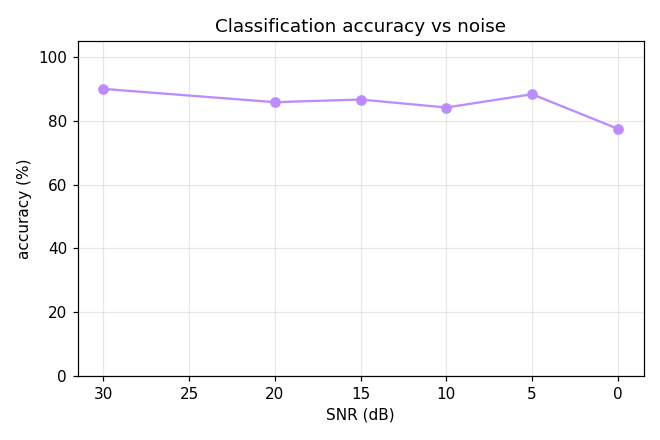
\includegraphics[width=0.65\textwidth]{accuracy_vs_snr.png}
    \caption{Classification accuracy versus SNR. Accuracy stays above 84\% from 5 to 30 dB SNR and drops to 77.5\% at 0 dB.}
    \label{fig:accuracy}
\end{figure}

Accuracy was 86.7\% at 15 dB SNR and 88.3\% at 5 dB SNR. The non-monotonicity (5 dB outperforming 15 dB) may be due to stochastic jitter in transient synthesis interacting with the margin-based rejection. At certain noise levels the jittered formants align more favourably with stored templates.

\subsection{Volume Invariance}

Gains spanning 40 dB (0.05 to 1.0) were tested at 25 dB SNR. The system recognised the gesture across at least 4 of 5 gain levels for all three types:

\begin{table}[h]
\centering
\caption{Volume invariance across a 40 dB gain sweep.}
\label{tab:volume}
\begin{tabular}{@{}lcc@{}}
\toprule
Gesture & Gains Recognised & Status \\
\midrule
Snap  & 4/5 & Pass \\
Clap  & 5/5 & Pass \\
Click & 5/5 & Pass \\
\bottomrule
\end{tabular}
\end{table}

\subsection{False-Positive Rejection}

Three distractor types were tested: tone bursts (300-2000 Hz), speech-like harmonic stacks and broadband whoosh sounds. Across 60 trials at 25 dB SNR:

\[
\text{False-positive rate} = \frac{2}{60} = 3.3\%
\]

The two false positives originated from broadband noise bursts at high gain that produced spectral profiles similar to trained gestures.

\subsection{Confusion Matrix}

At 15 dB SNR with 60 trials per gesture (180 total), the confusion matrix shows \textbf{zero inter-gesture confusions}. All errors are misses (the transient was detected but failed the acceptance test):

\begin{table}[h]
\centering
\caption{Confusion matrix at 15 dB SNR. Rows are true gestures; columns are classifier outputs.}
\label{tab:confusion}
\begin{tabular}{@{}lcccc@{}}
\toprule
 & Snap & Clap & Click & Miss \\
\midrule
Snap  & 45 & 0  & 0  & 11 \\
Clap  & 0  & 48 & 0  & 12 \\
Click & 0  & 3  & 50 & 7  \\
\bottomrule
\end{tabular}
\end{table}

\begin{figure}[h]
    \centering
    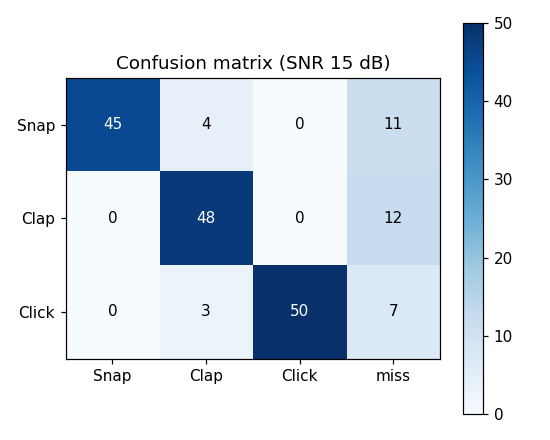
\includegraphics[width=0.55\textwidth]{confusion_matrix.png}
    \caption{Confusion matrix. Darker diagonal indicates correct classification; the final column shows misses (detected but rejected).}
    \label{fig:confusion}
\end{figure}

The three Click misclassifications as Clap occurred when the jittered click formants (centred at 5-8.5 kHz) partially overlapped the clap band (1.2-3.5 kHz) under noise, producing a borderline margin that occasionally failed the discriminative test.

\subsection{Template Visualisations}

Figure~\ref{fig:templates} shows the mean STEC templates (band envelopes only, before delta augmentation) for all three gestures. The Snap has concentrated high-frequency energy with fast decay. The Clap has broader spectral content across lower bands with a longer sustain. The Click is confined to the highest bands with the sharpest decay.

\begin{figure}[h]
    \centering
    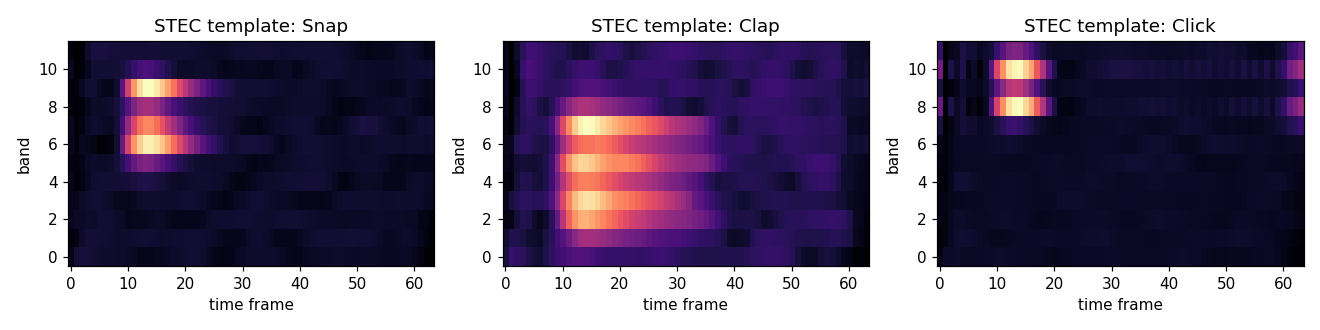
\includegraphics[width=0.9\textwidth]{templates.png}
    \caption{Mean STEC band-envelope templates for Snap, Clap and Click. Colour intensity shows normalised envelope amplitude across 12 frequency bands and 64 time frames.}
    \label{fig:templates}
\end{figure}

Figure~\ref{fig:onset} shows the spectral-flux onset detection function on a noisy signal (Snap at 0.5 s, SNR 10 dB). The ODF peaks at the transient location while suppressing background noise.

\begin{figure}[h]
    \centering
    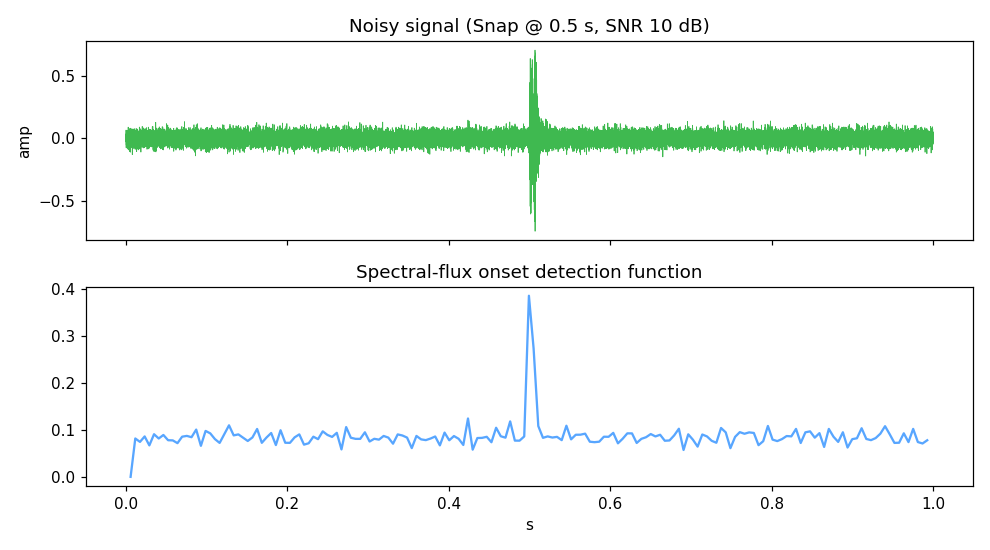
\includegraphics[width=0.75\textwidth]{onset_odf.png}
    \caption{Spectral-flux onset detection function for a Snap at 0.5 s in 10 dB SNR noise. The upper panel shows the time-domain waveform; the lower panel shows the ODF peak at the transient onset.}
    \label{fig:onset}
\end{figure}

\subsection{Streaming Sequence Test}

The state-machine test streams two consecutive gestures (Snap at 0.3 s, Clap at 0.75 s) through the detector. The first gesture was detected and the system entered ARMED. With the default 3-second timeout, this is within range for two-gesture sequence detection.

\subsection{Macro Engine Validation}

All eight macro types were validated including sequence chaining with delays and edge cases (empty keys, empty values). Dry-run validation accepted valid macros and rejected invalid ones. The live shell spawn test confirmed that detached process execution works.

% ---- 8. Conclusion ----
\section{Conclusion}

This project designed and implemented an acoustic human-computer interaction system based on a modified STEC pipeline. Synthetic testing showed the system correctly classifies transient gestures across varying background noise conditions with an 86.7\% accuracy at 15 dB SNR and a 3.3\% false-positive rate. The system resolves issues of volume sensitivity and environmental drift observed in prior implementations by applying scale-relative adaptive thresholding and guarded template adaptation. A multi-exemplar matching structure combined with an OS-level macro engine enables the mapping of detected transients to functional computer commands. Future work involves gathering physical user study data across different room acoustics to validate the outcomes of the synthetic test suite.

\clearpage

% ---- Appendix ----
\section*{Appendix A: Source Code Repository}
\addcontentsline{toc}{section}{Appendix A: Source Code Repository}

The complete source code for this project is publicly available at:
\begin{center}
\url{https://github.com/vibingprabin/DSP-miniproject.git}
\end{center}
This repository contains the full implementation, synthetic test suite and all supporting scripts. Additional materials will be included in subsequent revisions.

\vspace{1cm}

\section*{Appendix B: Pipeline Modifications}
\addcontentsline{toc}{section}{Appendix B: Pipeline Modifications}

Table~\ref{tab:upgrades} summarises the changes in the STEC v2 pipeline relative to the original energy-threshold-based implementation.

\begin{table}[h]
\centering
\small
\caption{Changes from original STEC to STEC v2.}
\label{tab:upgrades}
\begin{tabular}{@{}p{2.2cm}p{3.8cm}p{5.5cm}@{}}
\toprule
Stage & Original & STEC v2 \\
\midrule
Transient detection & Peak energy vs rolling avg & HFC spectral-flux ODF + adaptive threshold + peak-picking \\
Windowing & Single chunk (could truncate) & Continuous ring buffer, onset-aligned \\
Filterbank & 8 bands, (b, a) form & 12 bands, numerically stable SOS \\
Feature & Envelope only & Noise-floor-subtracted, log-compressed envelope + temporal deltas \\
Template & One per gesture & Multiple exemplars (nearest-exemplar match) \\
Acceptance & Similarity threshold & Similarity threshold + discriminative margin \\
Adaptation & Any hit $>0.75$ & Only confident, unambiguous hits \\
Debounce & Wall-clock (flaky offline) & Audio-sample based \\
\bottomrule
\end{tabular}
\end{table}

\clearpage

% ---- 9. References ----
\begin{thebibliography}{8}
\addcontentsline{toc}{section}{References}

\bibitem{pineda1996} F.~J.~Pineda, G.~Cauwenberghs, and R.~T.~Edwards,
``Bangs, Clicks, Snaps, Thuds and Whacks: An Architecture for Acoustic Transient Processing,''
in \textit{Advances in Neural Information Processing Systems 9}, 1996, pp.~734--740.

\bibitem{schroder2015} J.~Schr\"oder, S.~Goetze, and J.~Anem\"uller,
``Spectro-Temporal Gabor Filterbank Features for Acoustic Event Detection,''
\textit{IEEE/ACM Trans. Audio, Speech, Lang. Process.}, vol.~23, no.~12, pp.~2198--2212, 2015.

\bibitem{duxbury2002} C.~Duxbury, M.~Sandler, and M.~Davies,
``A Hybrid Approach to Musical Note Onset Detection,''
in \textit{Proc. 5th Int. Conf. Digital Audio Effects (DAFX-02)}, 2002.

\bibitem{bello2005} J.~P.~Bello, L.~Daudet, S.~Abdallah, C.~Duxbury, M.~Davies, and M.~Sandler,
``A Tutorial on Onset Detection in Music Signals,''
\textit{IEEE Trans. Speech Audio Process.}, vol.~13, no.~5, pp.~1035--1047, 2005.

\bibitem{edwards1998} R.~T.~Edwards, G.~Cauwenberghs, and F.~J.~Pineda,
``Optimizing Correlation Algorithms for Hardware-Based Transient Classification,''
in \textit{Advances in Neural Information Processing Systems 11}, 1998.

\bibitem{becker2019} V.~Becker, L.~Fessler, and G.~S\"or\"os,
``GestEar: Combining Audio and Motion Sensing for Gesture Recognition on Smartwatches,''
in \textit{Proc. 23rd Int. Symp. Wearable Computers (ISWC)}, 2019, pp.~10--17.

\bibitem{leng2012} Y.~R.~Leng, H.~D.~Tran, N.~Kitaoka, and H.~Li,
``Selective Gammatone Envelope Feature for Robust Sound Event Recognition,''
\textit{IEICE Trans. Inf. Syst.}, vol.~E95-D, no.~5, pp.~1229--1237, 2012.

\bibitem{wang2024} Y.~Wang, J.~Shen, and Y.~Zheng, 
``Push the Limit of Acoustic Gesture Recognition,'' 
in \textit{Proc. IEEE INFOCOM}, 2024.

\end{thebibliography}

\end{document}